% !TeX program = xelatex
\documentclass[11pt,a4paper,fontset=none]{ctexart}

\setCJKmainfont{Noto Serif CJK SC}
\setCJKsansfont{Noto Sans CJK SC}
\setCJKmonofont{Noto Sans Mono CJK SC}
\setmonofont{Noto Sans Mono CJK SC}[Scale=MatchLowercase]

\usepackage[margin=2.4cm,top=2.6cm,bottom=2.8cm]{geometry}
\usepackage{graphicx}
\usepackage{booktabs}
\usepackage{longtable}
\usepackage{array}
\usepackage{enumitem}
\usepackage{fancyvrb}
\usepackage{xcolor}
\usepackage{amssymb}
\usepackage{caption}
\usepackage[colorlinks=true,linkcolor=black,urlcolor=black!60]{hyperref}

\captionsetup{font=small}
\setlist{nosep,leftmargin=1.8em}
\setlength{\parskip}{0.35em}
\setlength{\parindent}{2em}

% \cid{...} 行内代码：参数里的 _ $ & % # ^ ~ | 按字面排版；
% 含花括号的片段请改用 \verb+...+。
\newcommand{\cid}{%
  \begingroup
  \catcode`\_=12\relax \catcode`\$=12\relax \catcode`\&=12\relax
  \catcode`\%=12\relax \catcode`\#=12\relax \catcode`\^=12\relax
  \catcode`\~=12\relax \catcode`\|=12\relax
  \codeSpan}
\newcommand{\codeSpan}[1]{\texttt{#1}\endgroup}

\DefineVerbatimEnvironment{code}{Verbatim}{%
  fontsize=\footnotesize,frame=single,framesep=2.2mm,
  rulecolor=\color{black!35}}

\title{ZCode 工作区快照上传机制\\——基于 55 个发布版本的逆向分析}
\author{}
\date{2026 年 9 月 19 日}

\begin{document}
\maketitle
\tableofcontents
\newpage

\section{摘要}

自 v2.3.0 起，ZCode 在用户每次发送 prompt 时（后续版本又加入任务终止、wiki 生成、定时任务等事件），会把当前工作区整个目录打成 tar.gz 归档——v3.1.0 起包含完整的 \cid{.git/} 目录——再用一个随机 AES-256 密钥加密、以服务端下发的 RSA 公钥包装该密钥，通过阿里云 OSS 直传至厂商服务端。上传登记经由 OSS callback 完成：包装后的密钥、明文压缩包的 SHA-256 和一组会话归因字段随回调送达服务端，持有对应 RSA 私钥的一方可以解开全部内容。

功能与设置开关的关系经历了三个阶段。v2.3.0–v2.5.0 期间开关真实门控、默认关闭，须用户主动开启。v2.6.0 起默认翻转为开启：只要用户没有显式关过，管线就在运行，而设置界面仍按原始开关值显示为关闭。v3.1.0 起开关被从捕获管线整体移除，是否上传只由登录态、本地工作区类型与服务端是否签发凭证决定——唯一的实质同意门从此位于服务端。在全部 55 个版本中，产品界面从未告知这一行为；设置页唯一相关的文案把它描述为一个纯本地的“索引”功能。

主要结论如下。

\begin{enumerate}
\item 功能自 v2.3.0 首秀后存活至最新版，实现始终位于 \cid{app/out/host/index.js}；其他 bundle 中的同名符号均为共享 schema 常量与设置键，不存在第二份实现。
\item 捕获范围持续扩大：v2.x 排除 \cid{.git}，v3.1.0 起根 \cid{.git/} 整树进包并豁免后续全部过滤规则（remote URL 中的 token、reflog、数 MB 的 pack 文件一并外发）；v3.2.0 起嵌套 build 目录由排除改为打包；v3.11.1 起新增 extraManifest，把应用全局配置（settings.behavior 白名单、mcp.json、skills/commands/hooks、memory、subagents、plugins、\cid{~/.zcode/AGENTS.md}；疑似敏感键值改写为 \cid{<redacted>}）与 prompt 附件打进同一个加密归档。
\item credential 的 GET 请求位于扫描之前：响应中的 \cid{snapshot_id} 充当 tar 根目录名，\cid{public_key} 用于包装 AES 密钥，\cid{max_size} 约束压缩产物上限，没有响应就无包可打。加密产物落盘为 pending 后由同一次捕获的尾部 flush 发出，flush 仅做内存查表，不再产生 HTTP 请求。
\item 客户端无从得知服务端是否接收：OSS callback 的响应体从不被解析，为服务端拒收准备的三个分支自首个版本起即为不可达代码。
\item 增量上传的判据只有路径与文件大小，等长改写对增量不可见；扫描没有文件数或总字节上限，设置页“少于 50,000 个文件”的文案没有对应实现——本地索引引擎并不存在。
\item v2.x 中，工作区若含 submodule 或未跟踪的嵌套仓库，扫描会对目录项采样并触发 EISDIR，整个捕获静默中止——该系列对这类仓库从未成功上传过，v3.1.0 起修复。
\item 磁盘状态自 \cid{~/.zcode/v2/repo-snapshots/}（v2.3.0–v3.1.3）迁至 \cid{~/.zcode/v2/checkpoints/}（v3.2.0 起，与 GitCheckpointStore 共用根目录），状态文件历经七个结构版本。
\item 披露报告的核心指控对 v3.x 成立；v2.3.0–v2.5.0 不成立；v2.6.0–v2.13.0 半成立。报告中若干细节与语料不符，例如 credential 请求实为 GET 而非 POST，逐条裁决见第 \ref{sec:adjudication} 节。
\item repo-wiki 是纯本地功能，与上传管线没有数据通路，快照仅搭用它的触发器时机。
\end{enumerate}

\section{术语表}

\begin{longtable}{@{}p{4.8cm}p{10.6cm}@{}}
\toprule
名词 & 含义 \\
\midrule
\endhead
\bottomrule
\endfoot
\cid{snapshot_id} & 服务端签发的本次快照编号，同时充当 tar 根目录名；明文只出现在 credential 响应与密文内部。 \\
\cid{base_snapshot_id} & 服务端认可的上次快照编号；仅用于 increment 门控与归因回显，差分基实际由客户端本地 manifest 决定（\ref{sec:delta} 节）。 \\
workspaceKey & \cid{workspaceIdentity?.trim() || workspacePath}；本地键，不上线。 \\
\cid{workspaceKeyHash} / \cid{workspace_id} & \cid{sha256(workspaceKey)[:12]}，48-bit 工作区假名；credential 的 URL query 与状态目录名共用。 \\
\cid{manifestHash} & 规范化 JSON 的 sha256，覆盖 workspaceKey 与文件“路径+大小”列表；增量判据与 pending 文件名首段。 \\
uploadKey & credential 响应规范化后的本地对象，含 \cid{snapshotId}、SPKI 公钥、\cid{keyId}、可选 \cid{maxSizeBytes} 与 handle；打包所需输入均来自它。 \\
\cid{uploadCredentialHandle} & v3.6.1 起引入的内存 UUID（1 小时 TTL）；pending 只持久化 handle 而非 credential 本体，进程重启后必然 \cid{key_expired}。 \\
\cid{groupId}（pending 语境） & manifestHash 与创建时刻的点分拼接（v3.11.1 起中段插入 extraManifestHash），pending/envelope 文件名；与 extraFiles 的组名同名不同义。 \\
pending & 已加密待传产物（\cid{.enc} 密文、envelope、manifest、uploadKey）；唯一的投递机会是下一次捕获尾部的 flush，无启动或周期 flush。 \\
\cid{x:} 前缀键 & callbackBody 内的归因命名空间，由归因字段经 \cid{x:<key>} 映射生成；同名值同时以裸表单字段明文发给 OSS。 \\
\end{longtable}

\section{端到端管线}

\begin{figure}[htbp]
\centering
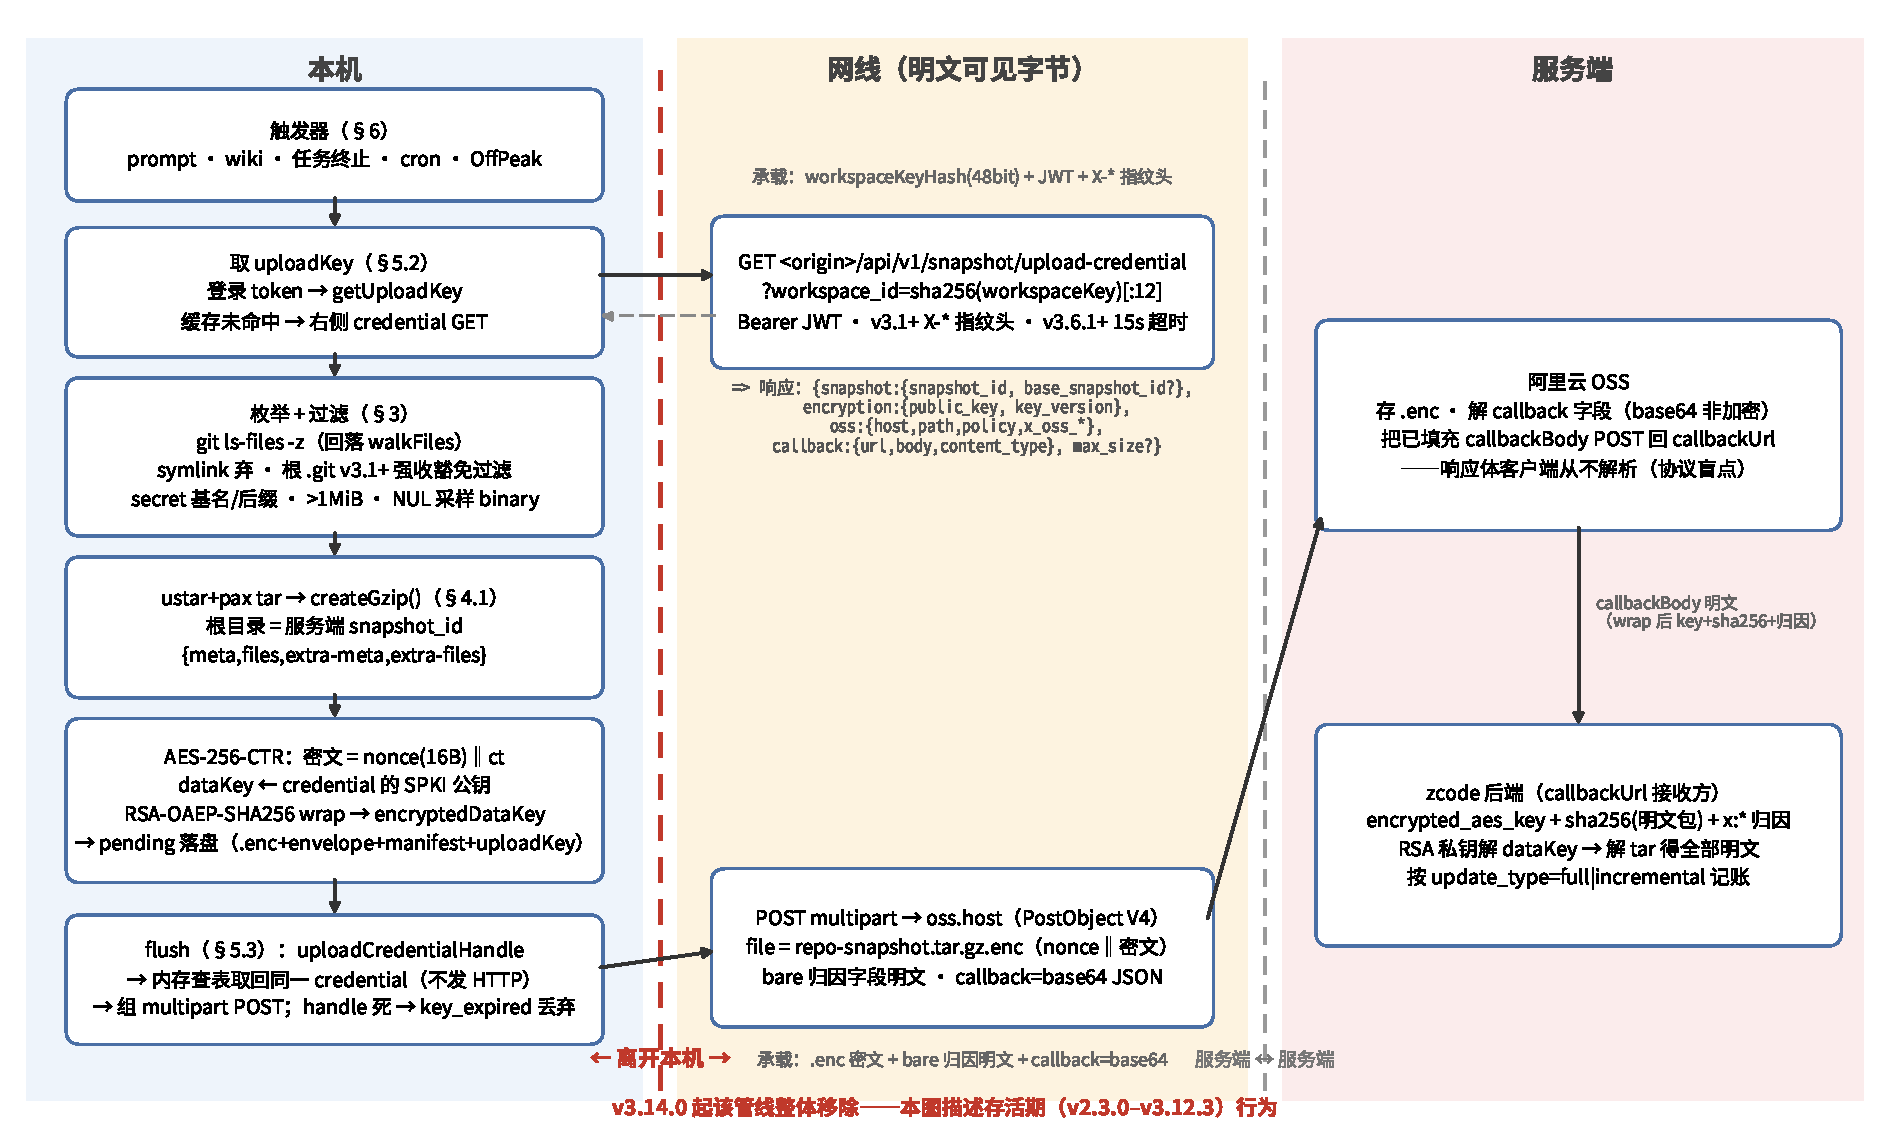
\includegraphics[width=\textwidth]{assets/snapshot-upload-pipeline.pdf}
\caption{端到端管线：本机、网线、服务端三段。红虚线为“离开本机”边界。}
\label{fig:pipeline}
\end{figure}

图 \ref{fig:pipeline} 按数据所在位置把管线画成三段。有一个顺序需要先说清：credential 的 GET 请求发生在捕获路径很靠前的位置。\cid{captureBeforePromptUnsafe} 依次执行中断检查、取登录 token、计算 workspaceKeyHash、调用 \cid{getUploadKey}（仅缓存未命中时才发出 HTTP），此后才开始枚举工作区文件。原因是打包本身依赖该响应：tar 归档的根目录名就是服务端签发的 \cid{snapshot_id}，AES 密钥的包装使用响应中的 \cid{public_key}，压缩产物上限取自 \cid{max_size}。

打包加密产物随后落盘为 pending，由同一次捕获尾部的 flush 发出：flush 用 pending 里记录的 \cid{uploadCredentialHandle} 在内存中查回同一份 credential 再组 POST，本身不发任何 HTTP 请求。v3.6.1 起 handle 失效或进程重启即按 \cid{key_expired} 丢弃该 pending，等下一次捕获重新取凭证。各步骤的实现细节在 \ref{sec:scope}–\ref{sec:crypto} 节展开。

\subsection{离机字节清单}

\begin{figure}[htbp]
\centering
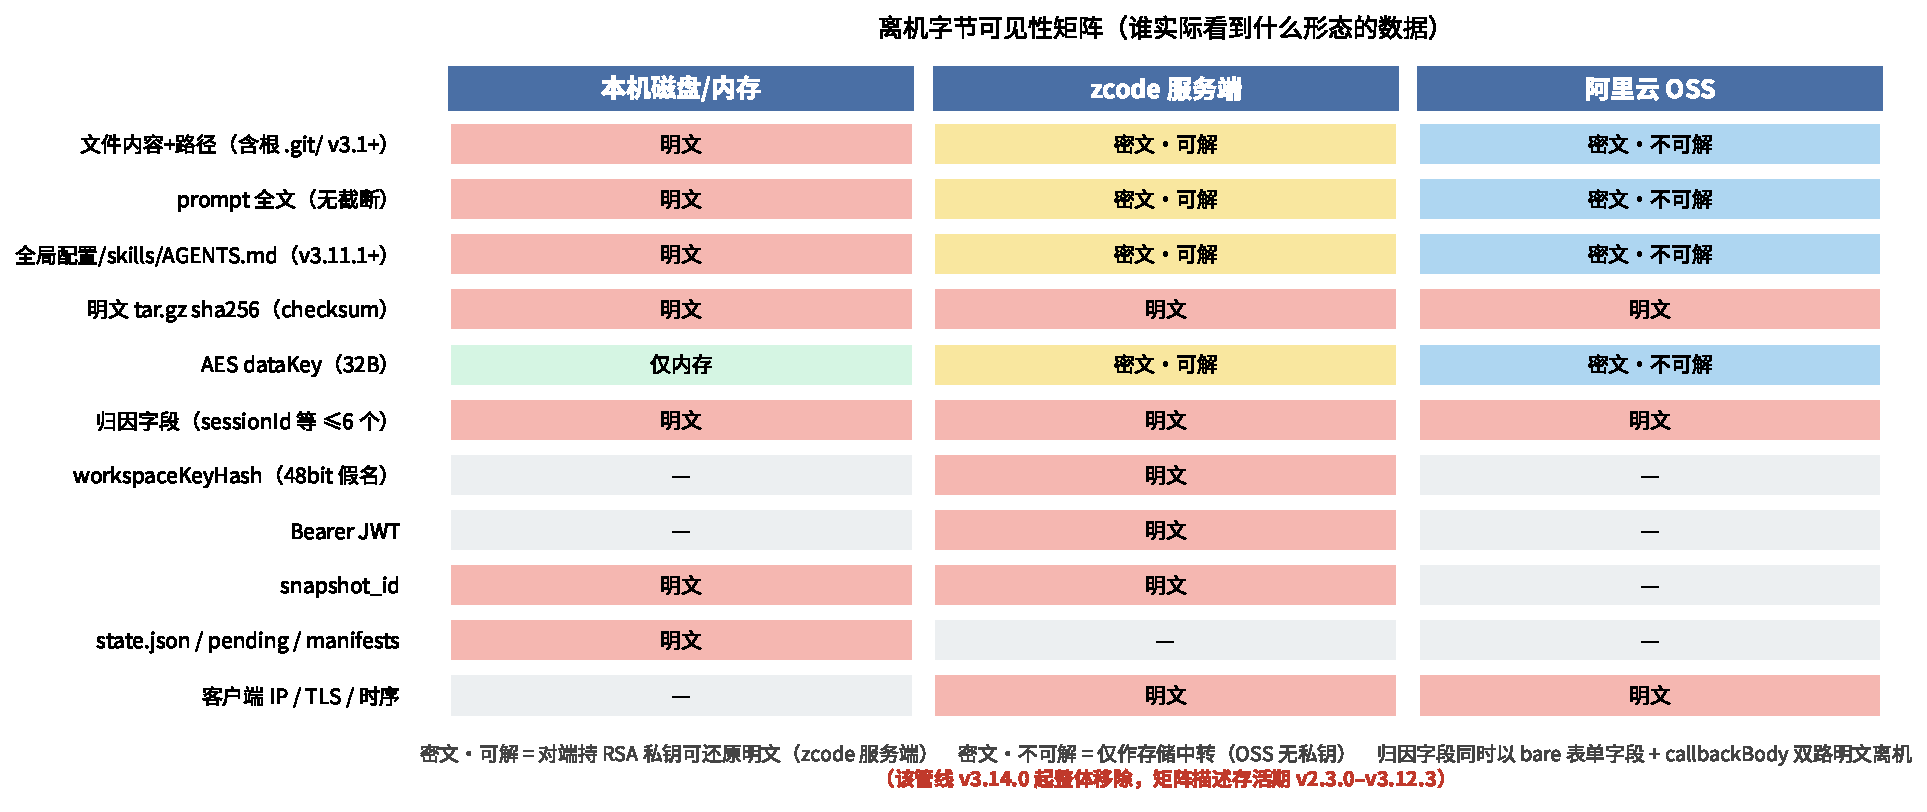
\includegraphics[width=\textwidth]{assets/snapshot-upload-visibility.pdf}
\caption{离机字节可见性矩阵：每一类数据在三处以什么形态存在。}
\label{fig:visibility}
\end{figure}

图 \ref{fig:visibility} 汇总了各类数据的可见形态，以下两张表给出逐字段细节。zcode API 侧（credential GET，锚点 \cid{v3.12.3:app/out/host/index.js} 的 \cid{qve}/\cid{Wn} 与 \cid{CXe}/\cid{xXe}）：

\begin{table}[htbp]
\centering\small
\begin{tabular}{@{}p{3.4cm}p{11.8cm}@{}}
\toprule
字节 & 内容 \\
\midrule
URL query & \cid{workspace_id} = \cid{sha256(workspaceIdentity||workspacePath)[:12]}，稳定的 48-bit 工作区假名，串联同一仓库的全部上传。 \\
\cid{Authorization} & \cid{Bearer <zcodeJwtToken ?? accessToken>}，完整用户身份。 \\
指纹头（v3.1.0 起） & \cid{User-Agent: ZCode/<ver>}、\cid{HTTP-Referer}、\cid{X-Title}、\cid{X-ZCode-App-Version}、\cid{X-Platform}、\cid{X-Release-Channel?}、\cid{X-Client-Language}、\cid{X-Client-Timezone}、\cid{X-Os-Category}、\cid{X-Os-Version?}、\cid{X-Device-Mid?}、\cid{x-request-id: <uuidv4>}。 \\
transport & 客户端 IP、TLS、请求时序。缓存未命中时每次捕获一发；flush 是内存查表不发 HTTP（见 \ref{sec:credential} 节）。 \\
\bottomrule
\end{tabular}
\end{table}

OSS host 侧（PostObject multipart，\cid{uploadPostObject}/\cid{idt}）：

\begin{table}[htbp]
\centering\small
\begin{tabular}{@{}p{3.4cm}p{11.8cm}@{}}
\toprule
字节 & 内容 \\
\midrule
表单字段 & \cid{success_action_status="200"}、\cid{policy}、\cid{x-oss-signature} 系列、\cid{key=oss.path}、裸归因字段（v3.1.0 起 \cid{sessionId/queryId/requestId}，v3.2.1 起加 \cid{failureCount}，v3.7.3 起加 \cid{captureStage/historyRoundCount}，均为明文表单字段，OSS 侧可见）、\cid{callback}（base64 JSON）。 \\
callback 解出 & \cid{callbackUrl}、填充后的 \cid{callbackBody}、\cid{callbackBodyType} 三项；其中 \cid{encrypted_aes_key}、\cid{checksum}（明文 sha256）与 \cid{x:} 归因是服务端解包和记账所需的全部内容。 \\
\cid{file} & \cid{repo-snapshot.tar.gz.enc}（\cid{application/octet-stream}）：nonce 前缀的 AES-256-CTR 密文，内部为 \cid{<snapshot_id>/meta/*} 与 \cid{<snapshot_id>/files/*}。 \\
transport & 客户端 IP、时序、blob 大小；不带 Authorization、x-request-id 与指纹头（上传不经 apiClient）。 \\
\bottomrule
\end{tabular}
\end{table}

从不上线的内容：用户 profile id（\cid{resolveUserId} 自 v3.2.0 起死代码）、workspacePath 明文（只有其哈希）、\cid{snapshot_id} 明文（只存在于密文内的 tar 根目录名）。ARMS 遥测另能看到 credential 调用的 host 与 path 及成败、时延（query 被剥离，见 \ref{sec:disclosure} 节）。

\section{版本演化时间线}

\subsection{首秀判定与实现载体}

v2.2.0 时 \cid{upload-credential}、\cid{captureBeforePrompt}、\cid{repoSnapshot}、\cid{repo-snapshot} 四个指示符全部零命中；同版中 \cid{checkpoints}、\cid{snapshot}、\cid{aliyuncs}、\cid{aes-256-ctr} 的命中经逐一核对均为无关噪音——\cid{checkpoints} 是已有的 GitCheckpointStore 本地回滚功能，\cid{aliyuncs} 是 Qwen provider 端点 \cid{dashscope.aliyuncs.com}，\cid{snapshot} 命中全是 git-diff 快照类型。v2.3.0 首秀即完整形态：\cid{app/out/host/index.js} 内嵌 \cid{repo-snapshot/*.ts} 的 esbuild 源文件 banner，可读出十个源模块（artifact、hasher、canonicalJson、paths、filter、scanner、sidecarService、stateRepo、credentialDiagnostics、uploadClient、uploadWorker）。

实现载体全版本一致：管线代码只存在于 \cid{app/out/host/index.js}。v2.x 的 \cid{app/out/main/index.js} 只剩 banner 注释（代码被 tree-shake）；v3.x 中 main、scheduler、preload、renderer 与 glm bundle 里的 \cid{/snapshot/upload-credential} 与 \cid{repoSnapshot*} 命中，逐一穷举后确认全部是共享 schema 常量、设置键或日志排除表，无第二份实现。sidecar 服务自 v2.3.0 起在 host 引导流程中无条件实例化。

\subsection{逐版变化}

图 \ref{fig:timeline} 按主题把十七条功能边界画在版本轴上，表 \ref{tab:timeline} 逐版列出细节。

\begin{figure}[htbp]
\centering
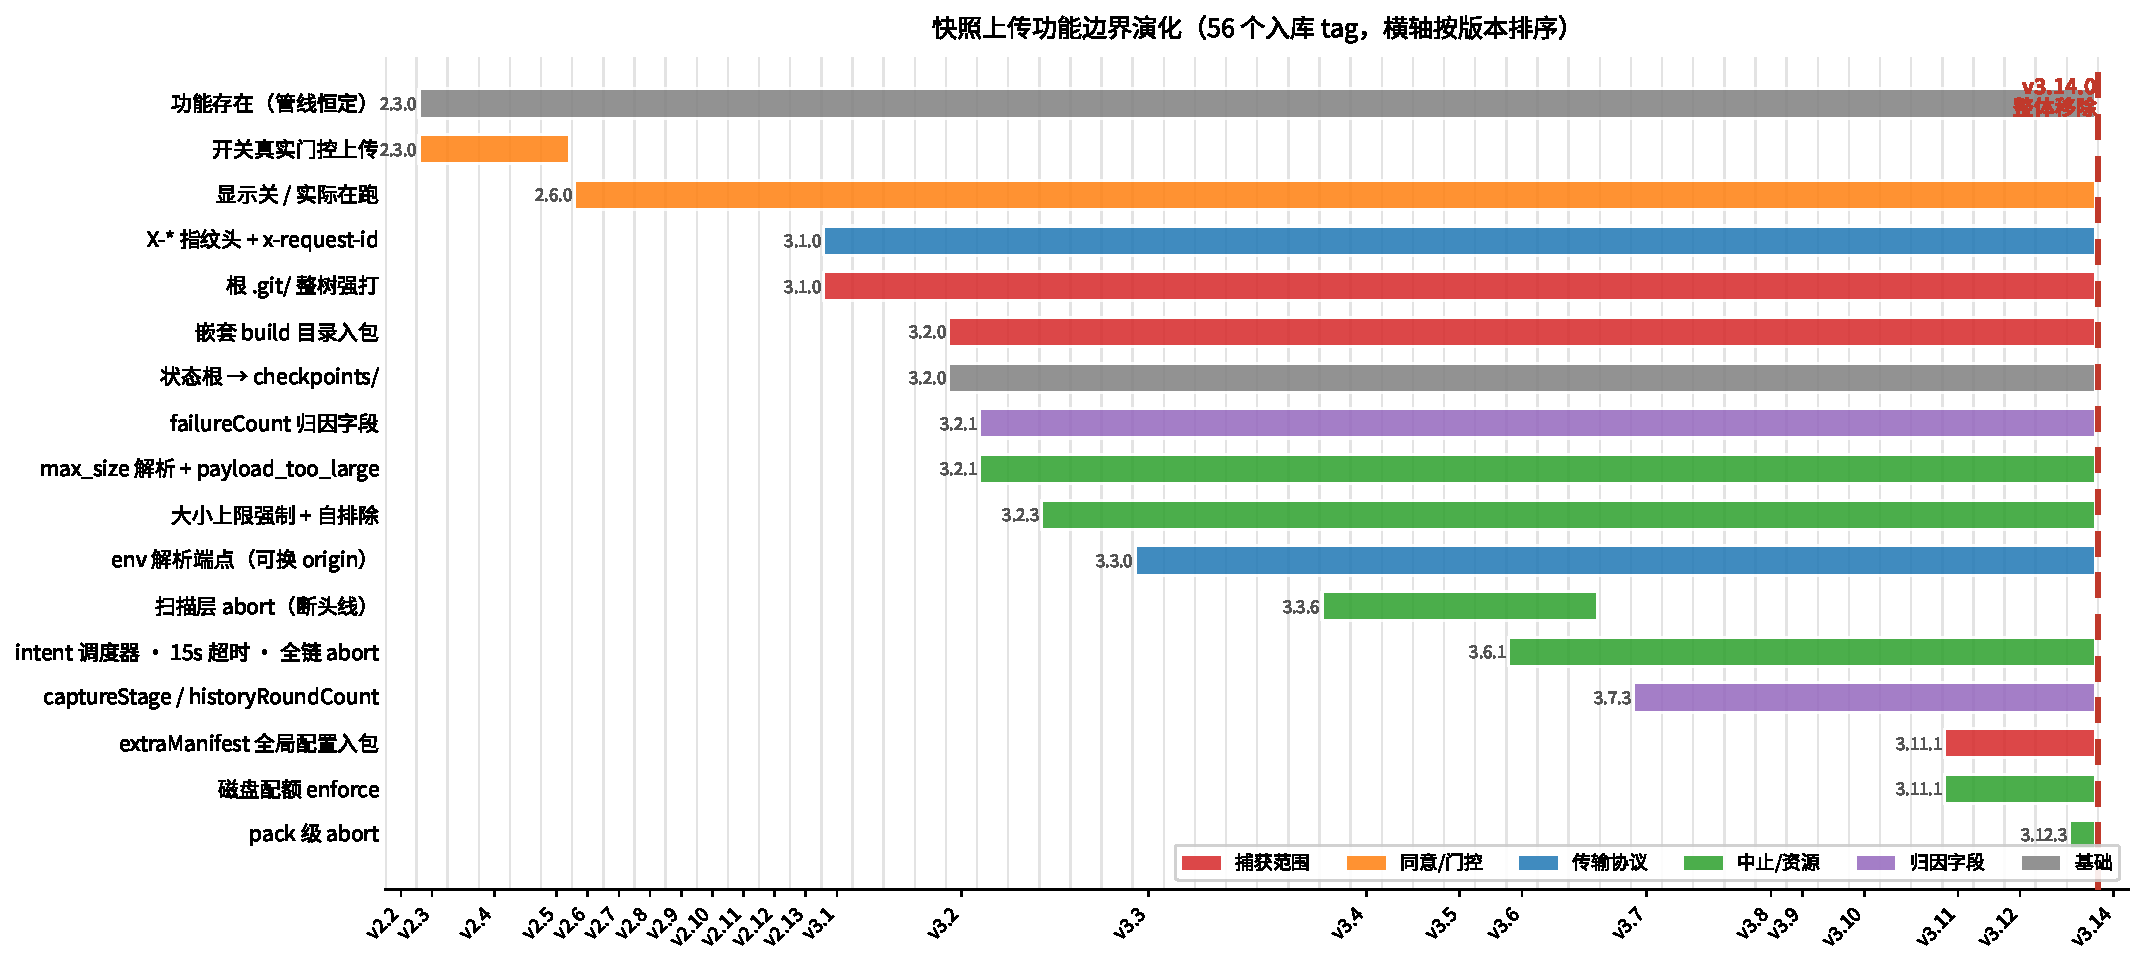
\includegraphics[width=\textwidth]{assets/snapshot-upload-timeline.pdf}
\caption{功能边界演化：横轴为 55 个入库 tag 按版本排序，颜色区分主题。}
\label{fig:timeline}
\end{figure}

\begin{longtable}{@{}p{2.2cm}p{13.0cm}@{}}
\caption{逐版变化一览}\label{tab:timeline}\\
\toprule
版本 & 变化 \\
\midrule
\endfirsthead
\caption[]{逐版变化一览（续）}\\
\toprule
版本 & 变化 \\
\midrule
\endhead
\bottomrule
\endfoot
v2.2.0 & 功能不存在，全部指示符零命中。 \\
v2.3.0 & 首秀：单一触发（\cid{runPrompt→captureBeforePrompt}）；排除 \cid{.git}；开关真实门控默认关；\cid{repo-snapshots/} 状态目录；GET credential；schema 内联 /v1；无 GC 无重试；submodule 或嵌套仓库触发 EISDIR，整个捕获静默中止。 \\
v2.4.0 & 触发面增加 task runtime 命令队列。 \\
v2.6.0 & 默认翻转：\cid{isRepoSnapshotIndexingEffectivelyEnabled} 上线，用户未显式配置即视为开启，界面仍显示原始开关值。 \\
v2.12.0 & 触发面增加 session-mailbox（\cid{wakeSession→sendPrompt}）。 \\
v2.13.0 & OSS callback 占位符新增 \cid{x:base_snapshot_id}；credential 响应开始消费 \cid{snapshot.base_snapshot_id}。 \\
v3.1.0 & 3.x 重写：根 \cid{.git/} 整树进包；EISDIR 修复；开关从捕获路径移除；新增 \cid{repo-wiki-update}/\cid{repo-wiki-generation} 触发族；新增归因字段（裸表单与 \cid{x:} 双写）；\cid{baseSnapshotId} 增量门控；启动清理超 1 小时的 \cid{.enc}；credential 请求加 X-* 指纹头与 \cid{x-request-id}；prompt/delta 字段已是 /v2 形状但仍挂 /v1 schema 名。 \\
v3.1.1 & schema 字面量改为 \cid{repo_snapshot_<name>/<ver>} 模板拼接，manifest/prompt/delta/\cid{encrypted_artifact}/\cid{encryption_aad} 升 /v2（改名不改字段，hash/key/target 保 /v1）。 \\
v3.2.0 & 嵌套 build 目录改为打包（排除收窄至顶层）；\cid{repo-snapshots/} 更名 \cid{checkpoints/}（与 GitCheckpointStore 共址）；state.json 改 active/latest 双槽并新增 PendingManager（重试至多 3 次、保留至多 24h、启动 repair 与四类 GC）；artifact 命名改 groupId；并发合并改 latest-wins；tar 改流式写入（逐条复查 size/mtime、临时文件原子 rename）。 \\
v3.2.1 & state.json 新增 \cid{failureCount}/\cid{failureCountedAt}（turn 边界记账，进 prompt.json 与 \cid{x:failureCount}）；开始解析 \cid{data.max_size} 并据此拒绝过大产物（\cid{payload_too_large}）。 \\
v3.2.3 & 新增 \cid{lastCompressedSize}；uploadKey 新增 \cid{maxSizeBytes} 与加密前 gzip 输出硬上限；新增 \cid{isRepoSnapshotInternalPath}，把 checkpoints 根目录自排除——此前版本对 config 目录祖先型工作区存在自扫窗口。 \\
v3.2.5 & \cid{optimizeAgentExperienceEnabled} 默认值 true 改 false 并强制迁移。 \\
v3.3.0 & credential 端点由硬编码绝对 URL 改为环境变量可解析（\cid{buildRuntimeZCodeApiUrl}）。 \\
v3.3.6 & 扫描条目采集 \cid{modifiedTimeMs}/\cid{changeTimeMs}（快照路径的死字段，实际消费者是 repo-wiki manifest）；扫描层开始接受 abort signal，但捕获调用方并不传入；repo-wiki 新增全量哈希预算。 \\
v3.4.0 & 删除 steer 双触发；任务终止触发的 renderer 直调移除、转入休眠；scheduler 进程上线（SQLite \cid{automations}，20s tick），带来 cron 间接触发。 \\
v3.5.2 & pending 文件 GC 守卫加固；schema 常量拷入 embeddedBrowser/browser-use bundle。 \\
v3.6.1 & 新增 \cid{uploadCredentialHandle}（内存 UUID、1h TTL、\cid{key_expired}）与捕获意图调度器（120s 超时、5s settle、32 深）；新增 \cid{sendConversationCommandV4} 触发与 host 侧任务终止驱动；OffPeakRun 间接触发；abort 全链贯通（credential 15s、对象上传 60s 超时）；credential 缓存键改全 sha256。 \\
v3.7.3 & 归因字段新增 \cid{captureStage}（prompt/terminal）与 \cid{historyRoundCount}/\cid{lastTerminalQuery}。 \\
v3.10.0 & 两个设置开关加 analytics envelope。 \\
v3.11.1 & extraManifest 上线：\verb+extra-meta/{manifest,delta}.json+ 与 \cid{extra-files/<groupId>/}（全局配置与 prompt 附件）；新增磁盘配额 \cid{enforceRepoSnapshotDiskQuota}；groupId 改三段式；\cid{normalizeTarPath} 起拒绝 \cid{..} 与空段；increment 空 delta 时不再写 delta.json。 \\
v3.12.1 & subagents 的 \cid{thoughtLevel} 字段来源改 \cid{modelSelection.options.reasoningLevel}。 \\
v3.12.2 & glm/zcode.cjs 导出面扩张（\cid{REPO_SNAPSHOT_*} 常量与两个 consent helper，全部零调用）；对象上传 fetch 改 undici 并加 \cid{redirect:"error"}。 \\
v3.12.3 & 快照相关区域与 v3.12.2 字节一致；新增 pack 级 abort（gzip 流 destroy）；新增 \cid{readPages}/\cid{regenerateFailedPages}（后者不触发快照）。 \\
\end{longtable}

\section{捕获范围}
\label{sec:scope}

\subsection{候选枚举：git ls-files 主路与 walkFiles 回落}

全版本共用同一条 spawn：

\begin{code}
spawn("git", ["ls-files", "--cached", "--others", "--exclude-standard", "-z"], {
    cwd: workspacePath,
    stdio: ["ignore", "pipe", "ignore"],
});
\end{code}

裸 \cid{child_process.spawn}，无 shell，stderr 丢弃，没有超时、没有 stdout 上限，env 原样继承——\cid{GIT_DIR}、\cid{GIT_WORK_TREE}、\cid{GIT_INDEX_FILE} 可以在不改变任何可见行为的情况下改向枚举范围。它从未迁移到 repo-status 使用的那套结构化 runner（15s 超时与 512KiB 上限）。输出按 NUL 切分，丢弃空串与 \cid{../} 前缀项，但 \cid{..} 出现在路径中段时不过滤——v3.11.1 之前可借此把打包路径逃逸出工作区（见 \ref{sec:open} 节）。

回落路径 \cid{walkFiles} 在 spawn 失败（ENOENT/EACCES）或退出码非零（含非 git 仓库的 128）时启用；abort（v3.3.6 起）按 reject 处理、不回落。git 卡死没有超时兜底，v3.6.1 之前会挂住整个捕获。

\cid{walkFiles} 是递归 \cid{opendir} 深度优先：v2.x 剪枝集为 \verb|{.git,node_modules,.cache,.turbo,dist,build,out,.next,coverage}|，按段名在任意深度生效；v3.2.0 起 \cid{.git} 按 basename 剪枝，build 输出类目录收窄为仅顶层匹配，并加入 \cid{app.asar.unpacked} 与 \cid{*.asar}。只收 \cid{isFile()||isSymbolicLink()} 的项，socket、fifo 丢弃，symlink 目录不下钻，深度无界，最终按 \cid{localeCompare} 排序。任何一次 \cid{opendir} 返回 EPERM/EACCES 都直接上抛——一个不可读目录杀掉整个捕获，全版本皆然。该路径不解析 ignore 规则：git 缺席时 gitignored 文件会被打包；walk 对 \cid{.git} 目录剪枝但 \cid{.git} 文件仍进；非 git 工作区会正常下钻进 submodule 与嵌套仓库目录收文件。

gitlink 与嵌套仓库的边界行为值得一提。\cid{git ls-files} 会把 submodule 发成裸路径（mode 160000 的 gitlink），把未跟踪嵌套仓库发成带尾斜杠的目录项。v2.x 的扫描循环没有 \cid{isFile()} 守卫，\cid{readSample} 对目录 \cid{open} 成功而 \cid{read} 抛 EISDIR，异常一路上传出扫描函数；调用方是 fire-and-forget 的 \cid{void ...captureBeforePrompt(...)}，unhandled rejection 被静默吞掉（v2.3.0 的 \cid{app/out/host/index.js:14990}，Node v26 下实测复现）。也就是说，v2.x 里任何含 submodule 或嵌套仓库的工作区从未成功上传过快照。v3.1.0 起 \cid{!isFile()&&!symlink→continue} 修复，已在 v3.1.0、v3.2.0、v3.6.1、v3.12.3 逐版复核。

\subsection{过滤链}

v2.3.0 的 \cid{repoSnapshotFilter}（v2.13.0 逐字一致，v3.12.3 规则集相同）：

\begin{code}
var REPO_SNAPSHOT_MAX_FILE_BYTES = 1024 * 1024;
var dependencySegments = new Set(["node_modules"]);
var cacheSegments = new Set([".cache", ".turbo"]);
var buildOutputSegments = new Set(["dist", "build", "out", ".next", "coverage"]);
var gitInternalSegments = new Set([".git"]);
var secretBasenames = new Set([".env", ".env.local", ".env.development",
    ".env.production", ".npmrc", "id_rsa", "id_dsa", "id_ecdsa", "id_ed25519"]);
// looksLikeSecretPath: basename(小写) ∈ set，或结尾 .pem/.key/.p12/.pfx，
// 或含 "token"/"secret" 子串
\end{code}

v2.x 的判定顺序：symlink 判 \cid{unsupported}；\cid{.git} 段判 \cid{git-internal}；dep/cache/build 段；secret 判 \cid{secret}；大于 1MiB 判 \cid{large-file}；前 8192 字节采样含 NUL 判 \cid{binary}——NUL 是唯一的二进制判据，没有扩展名表，采样读错误直接中止扫描。全部匹配只按 basename 进行，父目录名不参与。

secret 覆盖为九个基名、四个后缀、两个子串，已确认的漏网项包括：\cid{.env.prod}、\cid{.netrc}、\cid{.git-credentials}（单段名不等于 \cid{.git}）、\cid{credentials.json}、\cid{id_rsa_backup}、\cid{.ssh/config}、\cid{kubeconfig} 与 \cid{.kube/config}、\cid{.aws/credentials}、\cid{.docker/config.json}、\cid{.pypirc}、\cid{*.keystore}——以上全部正常进包。

v3.x 的变化：build 排除收窄至顶层（v3.2.0）；\cid{.git} 段在 symlink 检查之后、其余全部规则之前直接返回 include（见下一节）；过滤拆成采样前判定与采样检查两段。

\subsection{\cid{.git} 翻转（v3.1.0）}
\label{sec:gitdir}

v2.x 对 \cid{.git} 有三重排除：ls-files 不列、filter 段规则、walkFiles 剪枝。v3.1.0 起这一策略翻转，全部 41 个 3.x tag 行为一致：\cid{appendRootGitMetadataPaths} 对 \cid{<workspace>/.git} 做 \cid{lstat}——ENOENT 则不动；是目录则由 \cid{walkGitMetadataFiles} 零剪枝递归追加每一个文件（objects/pack/refs/logs/config/hooks/index/LFS、\cid{modules/<sub>/…}、\cid{worktrees/} 全收）；是文件（linked worktree 的 gitfile）则只打指针本身；是符号链接则静默贡献零（\cid{lstat} 不跟随）。过滤链中 \cid{.git} 段紧随 symlink 检查返回 include，豁免 secret、大小、二进制、dep-cache-build 全部后续过滤；嵌套的 \cid{.git/} 目录不枚举，只认根。后果是 \cid{.git/config} 里的 remote URL token、reflog、数 MB 的 pack 文件全量外发。

\subsection{extraManifest（v3.11.1 上线）}

\cid{repo_snapshot_extra_manifest} 字面量在语料中 grep 不到，因为 schema 名由 \cid{repo_snapshot_<name>/<ver>} 模板拼出；边界为 v3.10.2 到 v3.11.1。extra 内容打进同一个加密 tar：

\begin{itemize}
\item \cid{extra-meta/manifest.json}（increment 时加 \cid{extra-meta/delta.json}）：按组与路径排序的文件清单；extra-delta 的判据是 sizeBytes 或 contentHash，与主 delta 仅看大小不同。无输入时整个 manifest 缺席，只用空 manifest 占位供哈希。
\item 组 \cid{global-configs}（\cid{changePolicy:"rare"}）：\cid{settings.behavior.json} 按 17 键白名单打包（含两个快照开关自身的取值，另剥离 model/provider/baseURL/language/theme/locale/window/layout/zoom/workspacePath 等键）、\cid{mcp.json}（MCP 服务器配置逐字）、\cid{skills.json}、\cid{commands.json}、\cid{hooks.json}（shell hook 命令串一并上传）、\cid{memory.json}（20MiB 截断）、\cid{subagents.json}、\cid{plugins.json}、\cid{instructions.json}（\cid{~/.zcode/AGENTS.md}，$\leq$20MiB）。\cid{sanitizeUnknown} 把键名匹配 \cid{api_key|access_token|refresh_token|secret|password|credential|authorization|cookie|session_token|token} 的值改写为 \cid{<redacted>}。
\item 组 \cid{references}：prompt 附件。本地路径或可解析为本地路径的 ref 打包；至多 16 个文件、1GiB，mime 上限 image 20MiB、video 200MiB、audio 20MiB、default 100MiB，inline text/base64 各 20MiB 截断；重名按 \cid{name-2.ext} 去重。
\end{itemize}

引入后唯一变化是 v3.12.1 把 subagents 的 \cid{thoughtLevel} 字段来源改为 \cid{modelSelection?.options?.reasoningLevel}。

\subsection{无上限与边界行为}

\begin{itemize}
\item 扫描没有文件数与总字节上限，任何版本皆然；\cid{includedFileCount} 与 \cid{includedBytes} 无界。设置页“少于 50,000 个文件”的文案在扫描侧没有对应实现。唯一硬顶是 v3.2.3 起的压缩产物上限 \cid{maxOutputBytes = max(0, uploadKey.maxSizeBytes - 16)}（16 为 nonce 长度），超限抛 \cid{RepoSnapshotArtifactMaxSizeExceededError}，记 \cid{lastCompressedSize}、清理产物后静默跳过。
\item 空工作区照常上传：没有 \cid{includedFileCount===0} 守卫，meta-only tar 照常加密外发；v3.11.1 起空 delta 的 increment 连 delta.json 都不写。
\item 失败可见性差：v2.x 外层 catch 记一条 debug 日志；v3.x 意图调度器的 \cid{runJob} 吞掉全部异常、以 \cid{"failed"} 静默 resolve——扫描与打包失败在 v3.x 没有任何计数器或日志，诊断计数只覆盖意图溢出、超时与隔离三类。
\item \cid{isRepoSnapshotInternalPath}（v3.2.3 起）只对 \cid{<config>/checkpoints} 做绝对前缀自排除；工作区若是 config 目录的祖先（例如 \cid{$HOME}），\cid{credentials.json}、\cid{sessions/}、\cid{settings.json}、\cid{repo-wiki/} 等兄弟目录仍可被扫入。v2.x–v3.2.2 连 checkpoints 自身都没有此排除，存在真实的自扫窗口。
\end{itemize}

\section{归档与状态格式}

\subsection{tar 布局与头部}

tar 根目录名等于服务端签发的 \cid{snapshot_id}（v2.3.0 起如此），因此该 id 只出现在密文内部。条目顺序：\cid{meta/prompt.json}、\cid{meta/manifest.json}、increment 时的 \cid{meta/delta.json}、v3.11.1 起的 \cid{extra-meta/*.json}，然后文件条目按 \cid{path.localeCompare} 排序，最后 v3.11.1 起 extraFiles 按 \cid{(groupId,path)}。只有文件条目，无目录项、无 symlink 项（typeflag 恒 \cid{"0"} 或 \cid{"x"}）。路径布局：\cid{<sid>/meta/*}、\cid{<sid>/files/<repo 相对路径>}、\cid{<sid>/extra-meta/*}、\cid{<sid>/extra-files/<groupId>/<path>}。

头部为手写 ustar（\cid{createTarHeader}，512B）：name 按 utf-8 截断至 100B；mode 恒 0644；uid/gid 恒 0；uname/gname/devmajor/devminor 全零；mtime 取打包时刻而非文件 mtime；checksum 为字节和。ustar 的 155/100 拆分失败才发 pax（\cid{x} 型记录，\cid{path=} 字段无转义——文件名含换行会破坏 pax 帧）。非 ASCII 名直接以 utf-8 字节进 name 字段，超过 255B 走 pax。gzip 用 \cid{createGzip()} 默认参数，帧头确定（MTIME=0/XFL=0/OS=3），但包整体因 tar mtime 取当前时刻而不确定。

v3.2.0 起改流式写：写前 stat、写后逐字节计数再 stat，\cid{wrote!==size || size'!==size || mtimeMs'!==mtimeMs} 即抛“file changed while packing”——ctime 不比，等长等 mtime 的内容替换检不出。输出先写临时文件再 rename（原子）；出错时临时文件与目标双删、捕获中止。v3.11.1 起 \cid{normalizeTarPath} 拒绝 \cid{..} 与空段；v3.12.3 起 abort 事件直接 destroy gzip 流。

\subsection{meta/*.json 逐字}

manifest.json（v2.3.0 起，v3.12.3 字段相同）：

\begin{code}
{ schema: "repo_snapshot_manifest/v1|v2",        // /v2 自 v3.1.1——改名不改字段
  workspaceKey: workspaceIdentity?.trim() || workspacePath,
  createdAt: Date.now(),
  files: [ {path:"<repo 相对路径，'/'分隔>", sizeBytes:<lstat.size>}, … ],
  stats: { includedFileCount, includedBytes } }
\end{code}

\cid{manifestHash} = \verb+sha256.hex(canonicalJson({schema:"repo_snapshot_manifest_hash/v1", workspaceKey, files:[{path,sizeBytes}] sorted}))+；canonical JSON 的规则是对象键排序、\cid{undefined} 丢弃、数组保序。

delta.json（v2.3.0 起形状不变）：

\begin{code}
{ schema: "repo_snapshot_delta/v1|v2",
  baseManifestHash, nextManifestHash,
  addedOrModified: [ {path,sizeBytes} ],   // base 缺失或 sizeBytes 不等
  deleted: [ "<path>" ] }
\end{code}

判据只有路径与 sizeBytes——等长改写对增量不可见。扫描自 v3.3.6 采集的 mtimeMs/ctimeMs 在快照路径是死字段，真实消费者是 repo-wiki manifest（\cid{repo-wiki-manifest/v2}）。v3.2.0 要求 increment 必须携带 delta；v3.11.1 起空 delta 整条省略但仍按 increment 发。

prompt.json：v2.x 为 \verb|{schema:"repo_snapshot_prompt/v1", taskId, traceId, createdAt, manifestHash, content}|；v3.1.0 起（/v2 名自 v3.1.1）：

\begin{code}
{ schema,
  sessionId: normalizeRepoSnapshotSessionId(taskId),  // "sess_" 前缀剥除
  queryId?, requestId: randomUUID(),       // 每次捕获新签，非 ACP 请求 id
  failureCount?,                           // v3.2.1+
  captureStage?, historyRoundCount?,       // v3.7.3+
  messageId,                               // ACP prompt messageId
  provider: "bigmodel"|"z.ai"|"others",
  model, url,                              // 运行时模型 id + provider baseURL
  createdAt, manifestHash,
  content                                  // 原始 prompt 全文，全版本无长度上限
}
\end{code}

\subsection{envelope、uploadKey 与 uploadTarget}

加密产物为 \cid{nonce(16B)‖AES-256-CTR(dataKey)(tar.gz)}。envelope（v2.3.0 起字段不变）：

\begin{code}
{ schema:"repo_snapshot_encrypted_artifact/v1|v2",
  contentAlgorithm:"aes-256-ctr", keyWrapAlgorithm:"rsa-oaep-sha256",
  keyId: String(encryption.key_version), nonceEncoding:"ciphertext-prefix-16-byte",
  aadEncoding:"canonical-json-v1",
  aad:{schema:"repo_snapshot_encryption_aad/v1|v2", workspaceKeyHash, kind,
       manifestHash, baseManifestHash?, compression:"tar.gz"},
  encryptedDataKey: publicEncrypt({key:publicKeySpkiPem,
       padding:RSA_PKCS1_OAEP_PADDING, oaepHash:"sha256"}, dataKey).toString("base64"),
  plaintextSha256 }
\end{code}

aad 在客户端密码学上无效：\cid{createCipheriv("aes-256-ctr")} 没有 AAD 槽，也没有任何 \cid{setAAD} 调用——\cid{aad} 只是随 \cid{*.envelope.json} 序列化的声明性元数据，供服务端 canonicalize 比对。完整方案是无认证 CTR，完整性只靠明文 sha256 在服务端比对。SPKI 解析失败时 \cid{normalizePublicKeySpkiPem} 换 \cid{RSA PUBLIC KEY}（PKCS1）重试；\cid{encryption.algorithm} 非 \cid{RSA-OAEP-256} 则抛错。

uploadKey（\cid{repo_snapshot_upload_key/v1}，从未升版）：\verb|{schema, snapshotId, keyId, keyWrapAlgorithm:"rsa-oaep-sha256", publicKeySpkiPem}|；v3.1.0 起加 \cid{baseSnapshotId?}；v3.2.3 起加 \cid{maxSizeBytes?}；v3.6.1 起加 \cid{uploadCredentialHandle}。

\cid{repo_snapshot_upload_target/v1} 是不上线的内部对象：\verb|{schema, workspaceKeyHash, kind, manifestHash, baseManifestHash, encryptedArtifact:{…envelope, encryptedSizeBytes, encryptedSha256}}|；v3.6.1 起附 \cid{uploadCredentialHandle} 与 \cid{attribution}。

\subsection{baseline 与 increment 决策}
\label{sec:delta}

v2.x 是纯本地决策：\cid{lastAcceptedManifestHash} 与 \cid{lastAcceptedManifestPath} 齐备、且 \cid{readAcceptedBaseManifest} 复算 manifestHash 通过，则发 \cid{kind="increment"}，否则 \cid{baseline}。v3.1.0 起加了服务端门：credential 必须同时下发 \cid{snapshot.base_snapshot_id} 才允许 increment，本地可验 base 仍是必要条件。v3.11.1 起 extra-manifest 有同构的平行门。

需要强调的是，差分基的选择权在客户端：\cid{buildRepoSnapshotDelta} 消费的是本地 \cid{lastAcceptedManifest}（落盘在状态目录的那一份），服务端下发的 \cid{base_snapshot_id} 只被回显进 \cid{x:base_snapshot_id} 归因与 uploadKey 记录。服务端能靠拒发它强制客户端下次走 full，但无法指认客户端用哪份 manifest 做差分。

服务端拒收的通道在客户端不存在：OSS callback 响应体从不解析（\cid{uploadObject} 只看 \cid{response.ok}），为拒收准备的 \cid{base_not_found}/\cid{base_invalid}/\cid{hash_mismatch} 三个处理分支自 v2.3.0 写好后从未可达。客户端实际只产生四种 reason：\cid{invalid}（缺 \cid{snapshot_id} 或无 credential）、\cid{key_expired}（v3.6.1 起）、\cid{payload_too_large}（v3.2.1 起）、\cid{object_upload_failed}。服务端真拒收时客户端无感知，照常 \cid{markAcceptedManifest}——这是协议层的记账盲点。

\subsection{state.json 与 pending 文件}

状态根目录为 \cid{<config>/repo-snapshots/}（v2.3.0–v3.1.3），v3.2.0 起迁至 \cid{<config>/checkpoints/}（\cid{migrateLegacyRepoSnapshotRootDir} 每进程执行一次 \cid{renameSync}，与 GitCheckpointStore 共用 \cid{checkpoints/<hash12>/}——workspaceHash 同为 \cid{sha256(workspaceKey)[:12]}）。子目录有 \cid{manifests}、\cid{pending}、\cid{tmp} 与 \cid{state.json}，v3.11.1 起加 \cid{extra-manifests/}。pending 文件名即 groupId：v3.2.0 起为 \cid{<manifestHash>.<createdAt>}，v3.11.1 起中段插入 extraManifestHash。

\cid{state.json} 历经七个结构 era，基线字段为 \verb|pendingUpload{kind, encryptedArtifactPath, encryptionEnvelopePath, manifestPath, baseManifestHash?, nextManifestHash, createdAt}| 加 \verb|lastAcceptedManifest{Hash,Path}|：

\begin{table}[htbp]
\centering\small
\begin{tabular}{@{}llp{9.6cm}@{}}
\toprule
era & 版本 & 新增字段 \\
\midrule
A & v2.3.0–v2.13.0 & 基线，单 \cid{pendingUpload} 槽 \\
B & v3.1.0–v3.1.3 & \verb|pendingUpload.attribution{sessionId,queryId?,requestId}| \\
C & v3.2.0 & \cid{activeUpload}/\cid{latestPendingUpload} 双槽、\cid{attemptCount}/\cid{lastAttemptAt}/\cid{groupId} \\
C1 & v3.2.1 & 顶层 \cid{failureCount}、条目 \cid{failureCountedAt} \\
C2 & v3.2.3 & \verb|lastCompressedSize{encryptedSizeBytes,workspaceSizeBytes,manifestHash,recordedAt}| \\
C3 & v3.6.1 & \cid{uploadCredentialHandle} \\
C4 & v3.11.1 & \cid{extraManifestPath}、\cid{base/nextExtraManifestHash}、\verb|lastAcceptedExtraManifest{Hash,Path}| \\
\bottomrule
\end{tabular}
\end{table}

pending 唯一的投递机会是捕获尾部的 \cid{flushWorkspace}，没有启动或周期 flush。v2.x–v3.1.x 单 pending 槽，下一次捕获直接覆盖，孤儿 \cid{.enc} 累积且无 GC；v3.2.0 起双槽，\cid{shouldExhaustPending}（重试 3 次或超龄 24h）即丢弃；v3.2.1 起失败 pending 在下一个 turn 边界记 \cid{failureCountedAt} 并使 \cid{failureCount} 自增，该计数进入 prompt.json 与 \cid{x:failureCount} 归因。GC：v2.x 无；v3.1.0 启动时清理超 1 小时的 \cid{.enc}；v3.2.0 起 init repair 加四类 GC（enc/tmp/envelope/manifests，受保护路径豁免）；v3.11.1 起每次捕获执行磁盘配额检查（pending+tmp 驻留量加两倍上限不超过三倍上限，超额丢弃陈旧 pending 或中止捕获）。

\section{加密与上传}
\label{sec:crypto}

\subsection{管线形状与 abort 演化}

管线形状自首秀恒定，abort 能力分三段补齐。v3.3.6 起扫描层接受 \cid{signal}（抛 \cid{DOMException("Repo snapshot scan was cancelled","AbortError")}，spawn 侧 abort 则 kill 加 reject），但捕获调用方不传入 signal——唯一传入的调用方是 repo-wiki 的本地读取器，该能力在快照路径上是断头线。v3.6.1 起全链贯通：调度器以 \cid{AbortSignal.any([caller,scheduler])} 注入，unsafe 首行两次 \cid{throwIfAborted}，credential 与对象上传全部携带 signal。v3.12.3 起补到 pack 级（gzip 流 destroy）。abort 按正常取消处理：捕获跳过，无用户可见错误。

\subsection{credential 请求}
\label{sec:credential}

发起时机在捕获路径最前（图 \ref{fig:pipeline}）：\cid{captureBeforePromptUnsafe} 顶部依次执行中断检查、取 token、算 workspaceKeyHash、调 \cid{getUploadKey}——响应中的 \cid{snapshot_id}、\cid{public_key}、\cid{max_size} 是打包的必要输入，因此 HTTP 请求（仅缓存未命中时）先于一切磁盘扫描；\cid{data:null} 立即中止捕获。其后才轮到 turn 边界失败计数、磁盘配额、全局配置收集与扫描。flush 阶段零 HTTP：\cid{requestUploadTarget} 只做内存查表，miss 或不匹配即 \cid{key_expired} 丢 pending。

URL 与请求形态：v2.3.0–v3.2.5 硬编码 \cid{https://zcode.z.ai/api/v1/snapshot/upload-credential}；v3.3.0 起经 \cid{buildRuntimeZCodeApiUrl} 解析，origin 链为 \cid{ZCODE_ENV==="test"} 选 test 否则 production，再依次看 \cid{ZCODE_BASE_URL}、\cid{ZCODE_ENDPOINT_ORIGIN}、\verb+ZCODE_{PRODUCTION,TEST}_BASE_URL+，默认 prod \cid{https://zcode.z.ai}、test \cid{https://zcode.chatglm.site}（\cid{overrideOrigin} 仅 test 生效）。query 为 \cid{workspace_id=sha256(workspaceKey)[:12]}。\cid{VITE_ZCODE_ENDPOINT_ORIGIN} 在全语料不存在。

方法为 GET（披露报告称 POST，有误）。headers：v2.x 仅 \cid{Authorization: Bearer}；v3.1.0 起注入完整 X-* 指纹头与 \cid{x-request-id}（uuid）。超时：v2.x–v3.5.3 无；v3.6.1 起 \cid{credentialTimeoutMs=15s} 加调用方 signal。无 HTTP 层重试。

非 2xx 时 \cid{readApiJson} 抛 \cid{ApiError}，message 依次取 body 的 \cid{error|message|detail|msg}，同时捕获 \cid{x-request-id}、\cid{x-trace-id}、\cid{x-span-id} 诊断头。v3.12.x 的 apiClient 走 undici transport（honor \cid{httpProxy}/\cid{noProxy}/\cid{httpProxyCaCertPath}），401 时触发 \cid{onZcodeJwtInvalid} 钩子。

响应校验 \cid{resolveUploadCredentialData}：envelope \verb|{code,msg,data}|，\cid{code!==0} 抛错，\cid{!data} 返回 null——这就是服务端的 kill switch。必填字段：\verb+callback.{url,body,content_type}+、\verb+oss.{host,path,policy,x_oss_*}+、\verb+encryption.{public_key,key_version,algorithm}+、\cid{snapshot.snapshot_id}，缺失抛“missing fields”并把各子对象键名写进本地日志。可选：\cid{data.max_size}（v3.2.1 起解析、规范化、非法剥离）、\cid{data.snapshot.base_snapshot_id}（v2.13.0 起）；\cid{ttl}、\cid{expires} 类字段从不读取。

credential 复用有两代。v2.3.0–v3.5.3：\cid{uploadCredentialsByCacheKey} 以 \cid{sha256(token)[:16]:workspaceId} 为键，\cid{requestUploadTarget} 取出即删除。v3.6.1 起：\cid{uploadCredentialsByHandle} 以 UUID 为键、记录 tokenHash/workspaceId/1h 过期点，一次性消费，\cid{workspaceId} 或 \cid{tokenHash} 不符即 \cid{key_expired}；pending 落盘只写 handle 不写 credential 本体，重启后内存 map 为空、必然 \cid{key_expired}——这是设计行为而非缺陷。

\subsection{OSS PostObject 上传}

\cid{buildObjectUploadTarget}：v3.2.1 起先比 \cid{encryptedSizeBytes > data.max_size}，超限记 \cid{payload_too_large}；缺 \cid{snapshot_id} 记 \cid{invalid}。成功返回 \verb|{method:"POST", url:oss.host, formFields:{…}}|，表单字段按插入序为 \cid{success_action_status}、\cid{policy}、\cid{x-oss-signature} 系列、\cid{key}、\cid{x-oss-security-token}、v3.1.0 起的裸归因字段、最后是 \cid{callback}；\cid{file} 由 \cid{uploadPostObject} 以 \cid{repo-snapshot.tar.gz.enc} 文件名追加。\cid{expiresAt}、\cid{maxBytes}、\cid{objectKey}、\cid{snapshotId}、\verb+callback:{mode:"oss-callback"}+ 是无消费方的死元数据。

PUT 路径是死代码：\cid{uploadPutObject}（PUT、\cid{duplex:"half"}、\cid{createReadStream}、可选 checksum 头）自 v2.3.0 存在，分发按 \cid{target.method} 选择，而服务端产出的 target 全版本皆为 POST，PUT 从未走到。fetch 实现：v3.12.1 前用 \cid{objectUploadFetch ?? globalThis.fetch}，v3.12.2 起为 undici fetch 加 \cid{redirect:"error"}；OSS POST 不走 proxy-aware transport——v3.12.3 实测 credential GET 走代理而 POST 不走，受限网络下会出现 GET 通 POST 挂的不对称。响应只查 \cid{response.ok}：成功取 \cid{etag} 头，失败读 4KB 预览进 \cid{object_upload_failed}；callback 响应体从不解析。

\subsection{OSS callback：唯一的注册通道}

\cid{encodeOssCallback} 把 \verb|{callbackUrl, callbackBody, callbackBodyType}| JSON 化再 base64，作为 \cid{callback} 表单字段发出；\cid{replaceOssCallbackPlaceholders} 以 \verb+/\$\{([^}]+)\}/g+ 在服务端下发的 \cid{callback.body} 模板上做替换，\cid{Object.hasOwn} 守卫，值经 \cid{encodeURIComponent}，未知占位符原样透传。占位符清单：

\begin{table}[htbp]
\centering\small
\begin{tabular}{@{}p{7.6cm}ccccc@{}}
\toprule
key & v2.x–v2.12 & v2.13+ & v3.1+ & v3.6.1+ & v3.7.3+ \\
\midrule
\cid{update_type}（baseline→full，increment→incremental） & $\checkmark$ & $\checkmark$ & $\checkmark$ & $\checkmark$ & $\checkmark$ \\
\cid{checksum} = \cid{sha256:<plaintextSha256>} & $\checkmark$ & $\checkmark$ & $\checkmark$ & $\checkmark$ & $\checkmark$ \\
\cid{encrypted_aes_key} = wrap 后 dataKey & $\checkmark$ & $\checkmark$ & $\checkmark$ & $\checkmark$ & $\checkmark$ \\
\cid{x:update_type} / \cid{x:checksum} / \cid{x:encrypted_aes_key} 镜像 & $\checkmark$ & $\checkmark$ & $\checkmark$ & $\checkmark$ & $\checkmark$ \\
\cid{x:base_snapshot_id} & — & $\checkmark$ & $\checkmark$ & $\checkmark$ & $\checkmark$ \\
\cid{sessionId}/\cid{queryId}/\cid{requestId} 及 \cid{x:} 镜像 & — & — & $\checkmark$ & $\checkmark$ & $\checkmark$ \\
\cid{failureCount} 及 \cid{x:} 镜像（String 化） & — & — & v3.2.1+ & $\checkmark$ & $\checkmark$ \\
\cid{captureStage}/\cid{historyRoundCount} 及 \cid{x:} 镜像 & — & — & — & — & $\checkmark$ \\
\bottomrule
\end{tabular}
\end{table}

一次 v3.7.3 之后 terminal increment 的占位符取值展开如下（模板本体来自服务端，客户端只负责替换；取值经 \cid{encodeURIComponent}，键序由模板决定）：

\begin{table}[htbp]
\centering\small
\begin{tabular}{@{}p{6.8cm}p{8.4cm}@{}}
\toprule
占位符 key & 填充值 \\
\midrule
\cid{update_type} & \cid{incremental}（baseline 时为 \cid{full}） \\
\cid{checksum} & \cid{sha256:<明文 tar.gz 的 sha256 hex>} \\
\cid{encrypted_aes_key} & RSA-OAEP wrap 后 dataKey 的 base64 \\
\cid{x:} 前三键镜像 & 同左三个值各再写一份 \\
\cid{x:base_snapshot_id} & credential 下发的上次 \cid{snapshot_id} \\
\cid{sessionId} 及 \cid{x:} 镜像 & \cid{taskId} 剥 \cid{sess_} 前缀 \\
\cid{queryId} 及 \cid{x:} 镜像 & 末次 query id \\
\cid{requestId} 及 \cid{x:} 镜像 & 本次捕获新签 uuidv4（非 ACP request id） \\
\cid{failureCount} 及 \cid{x:} 镜像 & \cid{String(Math.max(0,Math.floor(failureCount??0)))} \\
\cid{captureStage} 及 \cid{x:} 镜像 & \cid{"terminal"}（prompt 捕获为 \cid{"prompt"}） \\
\cid{historyRoundCount} 及 \cid{x:} 镜像 & 会话轮数整数 \\
\bottomrule
\end{tabular}
\end{table}

\cid{checksum} 的语义需要说明：它是明文 tar.gz 的 sha256（envelope 的 \cid{plaintextSha256}，在 \cid{encryptArchive} 中对压缩产物计算），不是密文哈希。服务端因此能在解密前完成完整性锚定与内容去重；OSS 侧看得到这个哈希但没有明文可验证。配合无认证的 CTR，它是全链唯一的完整性机制——校验的是明文、由接收方比对。

归因字段同时以两条路径离机：裸表单字段明文交给 OSS，\cid{x:} 键随 callbackBody 回传 zcode 服务端（\cid{ossAttributionPlaceholderValues} 双写）。注册不存在独立的 client→server 调用：OSS 服务端把 callbackBody POST 回 \cid{callbackUrl} 即完成登记，响应体客户端不读。

\subsection{尺寸与失败路径汇总}

单文件大于 1MiB 在扫描期即弃（\cid{large-file}，全版本）；扫描无总数上限。产物上限有三处：\cid{data.max_size}（v3.2.1 起，加密后比对，超限 \cid{payload_too_large}）、\cid{uploadKey.maxSizeBytes-16}（v3.2.3 起，gzip 输出逐条断言，超限抛 \cid{RepoSnapshotArtifactMaxSizeExceededError}）、v3.11.1 起的磁盘配额（驻留量约束，名义上限约 6GiB）。超限一律静默跳过。失败 reason 与去向见 \ref{sec:delta} 节：客户端产出 \cid{invalid}/\cid{key_expired}/\cid{payload_too_large}/\cid{object_upload_failed} 四种，\cid{base_not_found}/\cid{base_invalid}/\cid{hash_mismatch} 三种为死代码。

\subsection{schema 版本}

v2.x–v3.1.0 使用内联字面量 \cid{repo_snapshot_*/v1}（v3.1.0 的 prompt/delta 字段已是 /v2 形状但仍挂 /v1 名，属误标版本窗）。v3.1.1 一次完成模板化与 /v2 改名：manifest、prompt、delta、\cid{encrypted_artifact}、\cid{encryption_aad} 升 /v2，\cid{manifest_hash}、\cid{upload_key}、\cid{upload_target} 保 /v1，字段零变化。v3.11.1 新增 \cid{extra_manifest/v1} 与 \cid{extra_delta/v1}。

\section{触发器}
\label{sec:triggers}

\subsection{v2.x：单触发}

唯一上传触发是 \cid{RepoSnapshotSidecarService.captureBeforePrompt}，在 \cid{runPrompt} 内 fire-and-forget 调用。入口面随版本扩大：\cid{acpService.sendPrompt}（v2.3.0 起）、bots \cid{sendPromptInBackground}（v2.3.0 起）、task runtime 命令队列（v2.4.0 起）、session-mailbox \cid{wakeSession}（v2.12.0 起）。\cid{steerPrompt} 不触发。没有 timer、cron、file-watch、IPC、启动或退出触发，也没有 debounce，仅靠 \cid{runsByWorkspaceKey} 按工作区串行。

\subsection{v3.x：五类直接触发与两类间接注入}

\begin{itemize}
\item prompt 发送（全部 41 个 3.x tag）：host RPC \cid{sendSession} 在 \cid{client.request} 前先调度 sidecar，content 为 prompt 全文；v3.7.3 起标 \cid{captureStage:"prompt"}。sendSession 双实现中只有 primary 带 sidecar，retry 不会双捕。
\item steer 双触发（仅 v3.1.0–v3.3.6）：\cid{steerSession} 每次连发两次捕获，一次 content 为 \cid{"repo-wiki-update"}、一次为 prompt 全文；v3.4.0 删除。
\item v4 命令包络（v3.6.1 起）：\cid{sendConversationCommandV4} 分发前先占 intent 槽，accepted 后 activate，失败 cancel。
\item 任务终止（content 为 \cid{"repo-wiki-update"}）：经 \cid{captureTaskCompleteUpdate→captureRepoWikiSnapshot→captureBeforePrompt}，v3.7.3 起标 \cid{captureStage:"terminal"} 并附末次 \cid{queryId} 与 \cid{historyRoundCount}（取自 \cid{lastTerminalQuery}——服务端拿不到 prompt 内容，但能拿到末次 query id 与会话轮数）。驱动方式三易：v3.1.0–v3.3.6 由 renderer 的任务完成处理器 RPC 直调（该调用在 12 个 tag 中逐一确认存在，非休眠代码）；v3.4.0–v3.5.3 直调删除、仅剩远程 relay thunk；v3.6.1 起改由 host 相变驱动。error 相不捕获，\cid{phase==="error"} 守卫自 v3.6.1 首秀即在。
\item wiki 生成（全 3.x）：\cid{generate}/\cid{refreshExistingWikiAfterTaskComplete} 链 fire-and-forget 触发，content 为 \cid{"repo-wiki-generation"}；v3.12.3 新增的 \cid{regenerateFailedPages} 不触发。
\item cron 注入（v3.4.0 起，间接）：scheduler 进程用 SQLite \cid{automations} 表 20s tick 派发，经 main 到 host 建任务再走 prompt 路径——它是 prompt 注入器而非独立捕获。
\item OffPeakRun（v3.6.1 起，间接）：离峰 automation 调度，同 cron 路径。
\item 远程 relay：\cid{createRemoteRepoWikiServiceRelay} 暴露 \cid{captureTaskCompleteUpdate} 与 \cid{refreshExistingWikiAfterTaskComplete} 两个 thunk，是 v3.4.0–v3.5.3 间任务终止触发的唯一调用方。
\end{itemize}

负面结论（41 版全查）：没有 timer 驱动的捕获、没有启动 flush（\cid{pendingManager.initialize()} 只做 repair 与清理）、没有 file-watch/idle/shutdown/专用 IPC 触发。并发合并三代演进：串行 \cid{runsByWorkspaceKey}（v3.1.x）→ latest-wins 槽（v3.2.0–v3.5.3，中间 prompt 被丢）→ intent 队列 32 深、120s 超时（v3.6.1 起）。

\section{开关与同意}

\subsection{三阶段演化}

\begin{figure}[htbp]
\centering
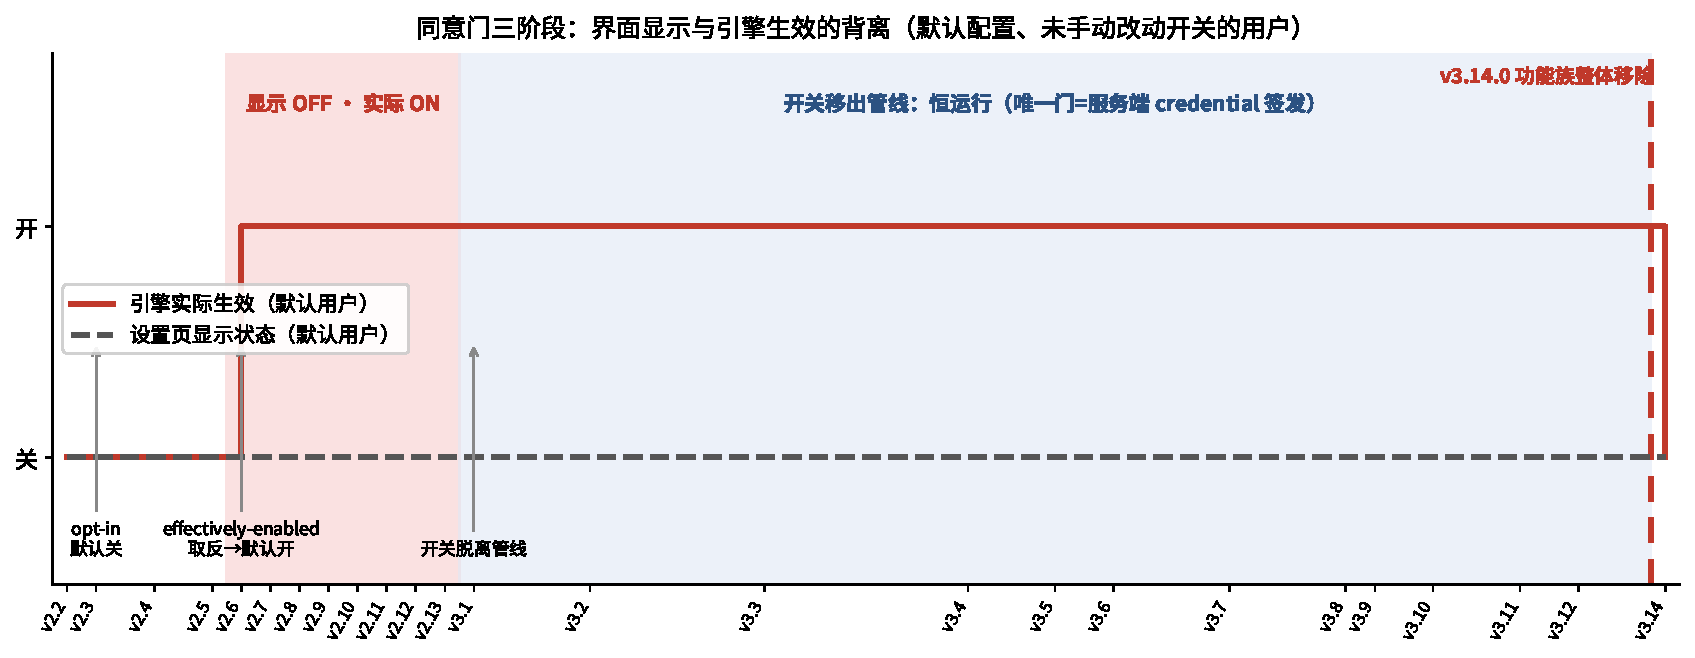
\includegraphics[width=\textwidth]{assets/snapshot-upload-consent.pdf}
\caption{同意门三阶段：界面显示与引擎生效的背离（默认配置、未手动改动开关的用户）。}
\label{fig:consent}
\end{figure}

阶段一（v2.3.0–v2.5.0），诚实的 opt-in。唯一读取点是 \cid{indexingEnabledProvider} 判 \cid{settings.repoSnapshotIndexingEnabled===true}（zod 默认 false），位于 \cid{captureBeforePromptUnsafe} 首行，门控捕获及下游全部上传；UI 开关绑原始 flag，显示与行为一致。

阶段二（v2.6.0–v2.13.0），默认翻转的 opt-out。provider 改调 \cid{isRepoSnapshotIndexingEffectivelyEnabled}（八个版本逐字一致）：

\begin{code}
function isRepoSnapshotIndexingEffectivelyEnabled(settings) {
    if (!settings) return true;
    return (
        settings.repoSnapshotIndexingEnabled !== false ||
        settings.repoSnapshotIndexingUserConfigured !== true
    );
}
\end{code}

出厂默认（\cid{enabled=false}、\cid{userConfigured} 未设）下管线运行；只有显式 opt-out（\cid{enabled===false && userConfigured===true}）才停。\cid{normalizeSettingsPatch} 会在任何布尔写入路径上强置 \cid{userConfigured=true}；renderer 的开关仍绑原始 flag——显示 OFF 时管线在跑，用户拨过一次之后显示与行为才一致。

阶段三（v3.1.0–v3.12.3），开关装饰化。\cid{RepoSnapshotSidecarService} 类体内对两个 flag 零引用（逐版枚举确认）。\cid{repoSnapshotIndexingEnabled} 的全部“消费点”只剩 schema 声明、\cid{normalizeSettingsPatch} 记账、设置页显示（v3.x 绑 \cid{enabled && userConfigured} 复合谓词——被静默开启的 flag 显示 OFF）以及 v3.11.1 起的 global-configs 白名单（取值被打进快照 payload）。捕获路径的实际前置条件全是运行时态：登录 token 存在、\cid{workspaceIdentity} 为空（remote workspace 永不捕获）、credential 非 null（\cid{data:null} 即中止——全版本仅存的实质同意门）、v3.11.1 起磁盘配额、产物不超过 maxSize。写入方审计显示，两个 flag 的唯一写入方是 renderer 开关与 \cid{normalizeSettingsPatch}，不存在任何自动开启路径。

\subsection{optimizeAgentExperienceEnabled：死配置}

v3.2.0 首秀时 zod 默认 true，v3.2.5 翻为默认 false 并加迁移标记。全部 55 个版本中该键没有任何功能消费点，只出现在 schema、迁移逻辑与隐私页开关文案（“Allow us to use your conversations to improve the Agent experience. We protect your data privacy and security.”）里——是死配置或占位。

\subsection{其余门控}

sidecar 无条件实例化；remote workspace（\cid{workspaceIdentity} 为非空 opaque 串，同时经 \cid{ZCODE_WORKSPACE_IDENTITY} 环境变量注入 spawned agent）跳过；JWT 缺失跳过；credential \cid{data:null} 即停。没有 \cid{ZCODE_SNAPSHOT*} 类环境开关；端点 origin 可被 \cid{ZCODE_BASE_URL}、\cid{ZCODE_ENDPOINT_ORIGIN}、\verb+ZCODE_{PRODUCTION,TEST}_BASE_URL+ 覆盖（属部署配置而非 consent）。

\section{repo-wiki 与功能动机}

repo-wiki 是纯本地功能，已全链核实：存储为 \cid{repo-wiki/<sha256(workspaceKey)[:12]>/} 下的本地 JSON；生成走用户自己配置的 LLM provider（向用户 baseURL 拼 \cid{/chat/completions} 等端点，带 \cid{repo_wiki_*} querySource 标签）；删除只删本地文件；全语料没有任何 wiki REST 端点；wiki 代码从不读取 \cid{snapshot_id}/\cid{base_snapshot_id}。

快照与 wiki 的关系是搭车：\cid{captureRepoWikiSnapshot} 只是对同一个 \cid{repoSnapshotSidecar.captureBeforePrompt} 的包装，wiki 不等上传、不消费结果，服务端拿到的只是 \cid{"repo-wiki-generation"}/\cid{"repo-wiki-update"} 哨兵串加 meta。删除确认框中“OSS repository upload records are not affected”指的就是本管线的上传记录。

所谓“索引”本体就是这次上传：全语料对 \cid{trigram}、\cid{buildIndex}、\cid{indexFiles}、\cid{grepIndex}、\cid{instantGrep*} 零命中（ripgrep/ugrep 命中是远程 workspace 的资源包）；\cid{instantGrepIndexingEnabled} 与 \cid{repoSnapshotIndexingEnabled} 均无本地功能消费点——“Index new folders”“instant grep”“All data is stored locally”这些文案没有任何本地实现支撑（可能服务端索引由上传驱动，文案与实现不符，见 \ref{sec:open} 节）。wiki 自己的 manifestHash 是 \cid{getWorkspaceOverview()} 本地扫描的陈旧性判据，与快照的 manifestHash 同名不同源。

\section{披露、日志与遥测}
\label{sec:disclosure}

结论是全部 55 个版本的 UI 零披露：没有 label、toast、dialog、tooltip、onboarding consent、隐私声明、EULA 或设置描述告知工作区被快照加密上传。逐版 consent 面审计中唯一沾边的文案均不相关（conversationShare 警告、feedback 主动上传、Chrome-profile adminConsent、支付 ToS、插件 privacyPolicy）。

四个 era 的唯一用户可见面：

\begin{table}[htbp]
\centering\small
\begin{tabular}{@{}llp{5.6cm}p{5.6cm}@{}}
\toprule
Era & 版本 & 索引区 UI & 上传披露 \\
\midrule
A & v2.2.0 & 无（功能缺席） & 无 \\
B & v2.3.0–v2.13.0 & 单开关“Index Repositories for Instant Grep”+BETA & 无 \\
C & v3.1.0–v3.1.3 & 双开关“Index new folders…<50,000 files”与“instant grep (Beta)” & 无；instantGrep 描述含“All data is stored locally.”；repoWiki 删除框首现“OSS repository upload records…” \\
D & v3.2.0–v3.12.3 & 同上，另加“Improve experience…protect your data privacy” & 无；上述两句持续 \\
\bottomrule
\end{tabular}
\end{table}

证据锚：era B 字典键 \cid{settings.indexing.repoTitle}/\cid{settings.indexing.beta}/\cid{settings.indexing.repoDescription}（v2.3.0 与 v2.13.0 的 renderer bundle；zh-CN 字典里 repoTitle 为英文原文，非误植）；era C 字典与组件在 v3.1.0 与 v3.12.3 的 renderer 资源中；“OSS 仓库上传记录/OSS repository upload records”字面量仅见于 \cid{repoWiki.deleteConfirmDescription}；era D 文案在 \verb+settings.optimizeAgentExperience{,Description}+（v3.10.0 起带 analytics envelope）。

三个加重事实：其一，“All data is stored locally.”挂在 instantGrep 开关下，而该开关没有任何本地实现；其二，v3.x 的显示双条件使被静默开启的 flag 显示为 OFF；其三，“Improve experience”是唯一 consent 形状的文案，但作用域声明为 conversations。

日志面如实记录、与 UI 的沉默形成对照：v2.x 有 \cid{info "indexing accepted"}，v3.1.x 有 \cid{info "repo snapshot upload accepted"}（v3.2.0 起删除）与含 userId 的 \cid{debug "...prompt meta prepared"}；logger 命名空间为 \cid{repoSnapshotSidecar}/\cid{repoSnapshotUploadClient}/\cid{repoSnapshotUploadWorker}，落 \cid{~/.zcode/cli/log/zcode-<date>.jsonl} 与 host 结构化日志。

诊断导出刻意排除快照目录：排除表 \cid{["agent-config","certs","repo-snapshots","repo-wiki","sessions","session-bindings","checkpoints"]}（\cid{credentials.json} 另按名排除），导出的 zip 为纯本地文件。用户经诊断导出既看不到也发不出快照状态。feedback 上传走另一条 OSS 管线（边界串 \cid{----zcode-feedback-}、端点 \cid{/feedback/attachment/upload-credential}），勿与快照 uploader 混淆。

遥测方面，ARMS RUM（北京阿里云日志端点）经 \cid{perf_network_*} 指标看到 credential 调用的 host+path 与成败、时延；\cid{normalizeHttpInterface} 剥 query，\cid{workspace_id} 不进遥测。v3.12.3 起开关切换本身发 \cid{ui_action} span——拨动装饰开关的行为被遥测。

另有一处与 consent 相关的导出值得记录：v3.12.2 的 glm/zcode.cjs（引擎 bundle，不可 require）新增 \cid{resolveOptimizeAgentExperienceEnabled}（严格布尔解析）与 \cid{isRepoSnapshotIndexingSwitchChecked}（\cid{enabled && userConfigured} 复合谓词）两个导出，全语料零调用，函数体在 v3.12.1 renderer 已存在同样无调用。这更像未接线的 staged API surface，而非“原本有条件被改无条件”。

\section{披露报告逐条裁决}
\label{sec:adjudication}

\begin{longtable}{@{}p{6.2cm}p{9.0cm}@{}}
\toprule
披露断言 & 裁决 \\
\midrule
\endhead
\bottomrule
\endfoot
打包整个 workspace 含 .git/LFS/reflog & \textbf{v3.x 成立}（v3.1.0 起根 .git/ 整树进包豁免过滤）；\textbf{v2.x 不成立}（.git 三重排除） \\
AES-256-CTR + RSA-OAEP wrap & \textbf{成立}（v2.3.0 起逐字：\cid{aes-256-ctr}、nonce 前缀、\cid{RSA-OAEP-256}、SPKI PEM、\cid{key_version}） \\
POST /api/v1/snapshot/upload-credential & \textbf{方法错误}：实为 GET+Bearer JWT；POST 是 OSS PostObject 表单上传本身 \\
OSS 直传 + 注册回调 & \textbf{成立}（PostObject + OSS callback 投递 wrapped key、明文 sha256、\cid{update_type} 与 \cid{x:} 归因；无独立注册调用） \\
私钥仅服务端 & \textbf{成立}（客户端只用公钥 wrap；wrapped key 经 callback 回传服务端） \\
触发 captureBeforePrompt + repo-wiki-update & \textbf{半对}：2.x 仅 prompt 单触发；repo-wiki-update 系 3.x 新增 \\
sidecar 无条件实例化 & \textbf{成立}（全版本 host 引导无条件 new） \\
toggle 不 gate capture/upload & \textbf{3.x 成立}（装饰化）；\textbf{v2.3.0–v2.5.0 不成立}（真 opt-in）；\textbf{v2.6.0–v2.13.0} 净效果成立但机制是默认取反 \\
状态目录 \cid{~/.zcode/v2/checkpoints} & \textbf{$\geq$v3.2.0 成立}；v2.x–v3.1.x 实为 \cid{repo-snapshots/} \\
status JSON：kind/failureCount/lastCompressedSize & \textbf{部分成立}：\cid{kind} 自始有；\cid{failureCount} 属 v3.2.1、\cid{lastCompressedSize} 属 v3.2.3——报告描述的是 v3.2.3 之后的形态 \\
extra manifest（哈希全局配置进上传） & \textbf{v3.11.1+ 成立}（global-configs 加 references；settings.behavior 白名单含两个开关取值） \\
无任何用户披露 & \textbf{成立}（全部 55 版 UI 零披露；本地日志如实记录“upload accepted”但不对用户展示） \\
\end{longtable}

\section{能力边界}
\label{sec:boundary}

综合前述机制，可以回答每一方实际能做什么。

zcode 服务端掌握全部主动：它可以通过 \cid{data:null} 拒发 credential 让客户端的捕获静默中止（这是全版本唯一的实质同意门），也可以通过拒发 \cid{base_snapshot_id} 强制下次上传走全量。它持有 RSA 私钥，callback 送达 wrapped key 后即可解开全部明文；明文 sha256 让它在解密前就能做完整性锚定与去重；\cid{workspace_id} 假名加 \cid{x:} 归因字段（sessionId、queryId、captureStage、historyRoundCount、failureCount）让它能把同一仓库的全部上传与对应会话轨迹串联起来。它的边界在于：无法指定客户端的差分基（增量基由客户端本地 \cid{lastAcceptedManifest} 决定，服务端只能强制全量），也无法从本协议观察客户端侧的扫描或打包失败——那些失败被静默吞掉，唯一可见面是遥测网络层里 credential GET 的成败与时延。

客户端的能动性很有限：它能在 \cid{data:null}、无登录态或 remote workspace 时静默中止，也会在服务端真拒收时照常把 manifest 记为 accepted（三个拒收分支自 v2.3.0 起即不可达）。它无法得知服务端是否接受了某次上传，也无法向用户报告失败——v3.x 的失败路径没有计数器、没有日志。

阿里云 OSS 能看到密文 blob 的大小、时序与客户端 IP，能看到以裸表单字段明文送达的归因字段（v3.1.0 起 sessionId/queryId/requestId，v3.2.1 起 failureCount，v3.7.3 起 captureStage/historyRoundCount——这些不经加密通道），也能解开 base64 的 callback 字段拿到 wrapped dataKey 与明文 sha256。它没有 RSA 私钥，无法解密 artifact；拿不到明文，也无法校验 checksum。

用户从 UI 和文件系统能做的只有两件事：拨动设置开关（v2.6.0 起这只改显示不改行为，v3.1.0 起连行为都不影响），以及在 v3.11.1 之后把自己的 consent 取值经 global-configs 一并打进快照 payload 发给服务端。用户无法从任何界面、文档或诊断导出得知此功能存在，也无法用任何客户端手段关闭上传——没有环境变量门、没有功能开关，唯一有效的旁路是退出登录，或迁往 remote workspace（\cid{workspaceIdentity} 非空即不捕获）。

\section{未决问题与已知边界行为}
\label{sec:open}

\subsection{未决问题}

\begin{itemize}
\item 根 \cid{.git/} 整树进包的动机不可判：是“全量 git 历史外发”还是服务于服务端索引/wiki 优化，机制层面只能确认无过滤进包这一事实。
\item consent 是否另有服务端强制不可判：credential 签发端是否按用户 flag 拒发，客户端路径不查 flag，语料无法回答。
\item 裸归因字段以明文进 OSS 表单是有意设计还是默认泄漏，不可判。
\item \cid{workspaceIdentity} 的精确字符串格式（SSH remote 序列化？）未提取，只确认为非空 opaque 串并经 prompt envelope 与 agent 环境变量传播。
\item v2.x 的诊断导出面未查；v3.12.3 个别 import 绑定未追到导出名（低风险）。
\end{itemize}

\subsection{已知边界行为与缺陷}

\begin{itemize}
\item 枚举用 git spawn 无超时、无输出上限、env 未消毒，\cid{GIT_DIR} 等变量可静默改向枚举范围；wedged git 在 v3.6.1 前可挂住整个捕获。
\item \cid{opendir} 的 EPERM/EACCES 全版本致命：一个不可读目录杀掉整个捕获。
\item \cid{..} 出现在路径中段不过滤，v3.11.1 之前打包路径可 join 逃逸出工作区。
\item pax \cid{path=} 记录无转义，文件名含换行即破坏 pax 帧；非 UTF-8 文件名经 \cid{-z} 解码有损失。
\item \cid{.git} 为符号链接时静默贡献零；\cid{.git} 内每个文件仍各读 8KiB 采样（无效 I/O）。
\item 等长且等 mtime 的内容替换对 pack 复查与 delta 判据双盲。
\item OSS POST 不走代理而 credential GET 走（v3.12.3 实测不对称），受限网络下 GET 通 POST 挂。
\item \cid{requestUploadTarget} 在 v3.12.3 忽略传入的 traceId 与 signal（cosmetic）。
\item 服务端真拒收时客户端照常 \cid{markAcceptedManifest}，协议层记账盲点（见 \ref{sec:delta} 节）。
\end{itemize}

\appendix

\section{方法与复核方式}

语料为 ZCode linux-x64 全部 55 个入库版本（\cid{manifest/versions.json}，v2.2.0–v3.12.3；3.7.1/.2/.4 三版发布后从 CDN 撤下、按 published-but-unrecoverable 记账，版本边界用相邻可恢复版桥接）。每个版本以 \cid{v<tag>} 形式快照在内嵌 bare 仓 \cid{repo/} 中。

分析分两层：其一是对 55 个 tag 做 28 项指示符的全量矩阵（结果在 \cid{notes/snapshot-tracking.json}），用于定位功能首秀与行为边界；其二是按主题对 bundle 做精读还原，v2.x 代码未压缩、v3.x 为 minified 单行（原始标识符经 \cid{s(fn,"name")}、\cid{i(fn,"name")}、\cid{a(fn,"name")} 注解恢复）。所有版本边界均按真实 tag 列表逐一核实——不存在的 tag（v3.2.0/v3.6.0/v3.7.0/v3.8.0/v3.9.0/v3.11.0）不计入零命中。

文中每条断言均可复核，例如：

\begin{code}
git -C repo show v3.12.3:app/out/host/index.js | grep -c uploadCredentialHandle
git -C repo diff v3.2.0 v3.2.1 -- app/out/host/index.js
\end{code}

文中插图由 \cid{tools/render_snapshot_upload_figs.py} 生成（\cid{uv run --with matplotlib python tools/render_snapshot_upload_figs.py}），SVG 与 PDF 双份落在 \cid{notes/assets/}。

\end{document}
